% Pipeline figure for the Semantic Recall metric, in the style of
% paper/system_fig/system_overview.tex.
%   Archive images + THINGS nouns --> joint SigLIP2 text-image embedding -->
%   for each noun, the nearest archive image --> Semantic Recall score.
% Image/score assets + _recall_meta.tex built by tools/build_metric_fig_assets.py.
% Compile: pdflatex semantic_recall.tex
\documentclass[border=8pt, varwidth=false]{standalone}
% Shared TikZ styling for the eval-metric pipeline figures, matching the look of
% paper/system_fig/system_overview.tex. \input after \documentclass{standalone}.
\usepackage{tikz}
\usetikzlibrary{positioning,shapes.geometric,arrows.meta,calc,fit,backgrounds,fadings}
\usepackage{graphicx}
\usepackage{amsmath,amssymb}
\usepackage{xcolor}
\usepackage[T1]{fontenc}

\tikzset{
  >=Stealth,
  box/.style       = {draw, rounded corners=2pt, align=center,
                      inner sep=4pt, line width=0.6pt, fill=white},
  vlmbox/.style    = {box, fill=blue!5,    draw=blue!55!black},
  embbox/.style    = {box, fill=violet!7,  draw=violet!60!black},
  databox/.style   = {box, fill=black!3,   draw=black!45},
  scorebox/.style  = {box, fill=orange!12, draw=orange!75!black, line width=0.9pt},
  img/.style       = {draw=black!45, line width=0.4pt, inner sep=0, outer sep=0},
  pipe/.style      = {->, line width=0.7pt, draw=black!75},
  feed/.style      = {->, line width=0.9pt, draw=orange!75!black},
  frame/.style     = {draw=black!45, line width=0.5pt, rounded corners=4pt,
                      inner sep=10pt},
  colTitle/.style  = {font=\bfseries, anchor=south west},
}


% Featured-run metadata (regenerated by tools/build_metric_fig_assets.py).
\IfFileExists{_recall_meta.tex}{% auto-generated by tools/build_metric_fig_assets.py
\def\recallCells{0/cockatoo/0.151, 1/teapot/0.146, 2/parrot/0.145, 3/eye/0.143, 4/kettle/0.141, 5/owl/0.140}
\def\recallScore{0.087}
\def\recallNumNouns{1{,}823}
}{%
  \def\recallCells{0/cockatoo/0.151, 1/teapot/0.146, 2/parrot/0.145,
                   3/eye/0.143, 4/kettle/0.141, 5/owl/0.140}%
  \def\recallScore{0.087}\def\recallNumNouns{1{,}823}%
}

\begin{document}
\begin{tikzpicture}[font=\footnotesize, x=1cm, y=1cm]

% ===================== SOURCE: ARCHIVE =====================
\node[frame, minimum width=4.6cm, minimum height=4.6cm, anchor=north west]
  (arch) at (0,0) {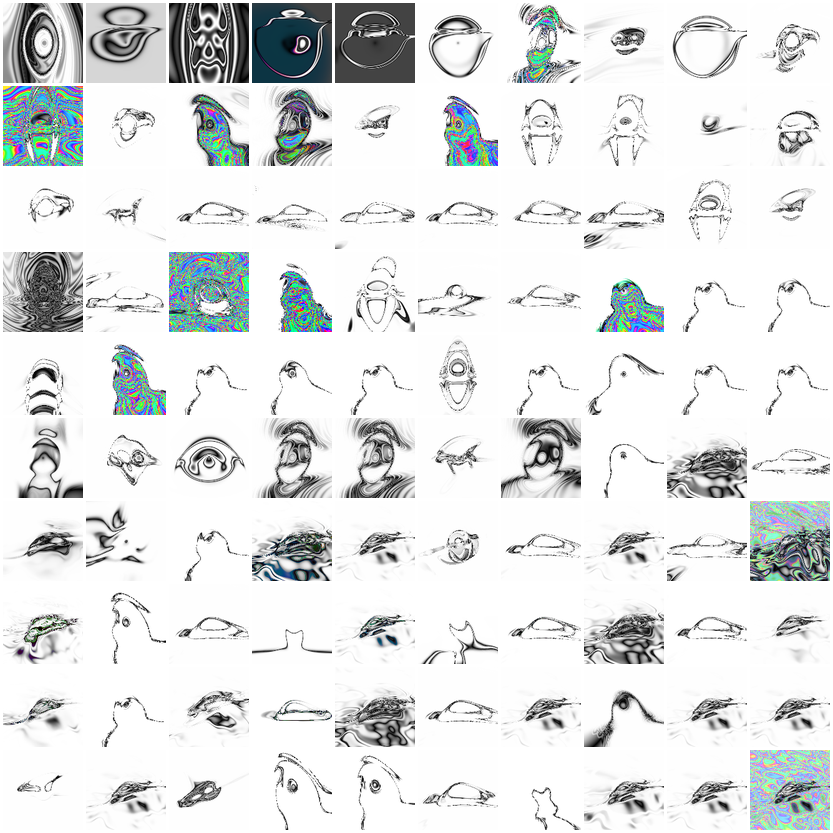
\includegraphics[width=4.0cm]{archive_grid.png}};
\node[colTitle] at (arch.north west) {Archive};

% ===================== SOURCE: THINGS NOUNS =====================
\node[databox, anchor=north, text width=3.9cm, align=center]
  (nouns) at ([yshift=-0.7cm]arch.south) {%
  \textbf{THINGS nouns} (\recallNumNouns)\\[2pt]
  {\itshape\scriptsize duck, teapot, eye, car,\\ owl, dolphin, parrot, \dots}};

% ===================== EMBED =====================
\node[embbox, anchor=west, text width=2.3cm]
  (emb) at (5.9,-2.3) {SigLIP2\\ text\,+\,image\\ embedding};
\draw[feed] (arch.east) -- node[above, font=\scriptsize] {images} (arch.east -| emb.west);
\draw[feed] (nouns.east) -| ([xshift=-0.7cm]emb.west)
            node[pos=0.25, below, font=\scriptsize] {text} -- (emb.west);

% ===================== MATCHING PANEL =====================
\node[frame, anchor=north west, minimum width=8.6cm, minimum height=4.6cm]
  (match) at (9.7,0) {};
\node[colTitle, align=left] at (match.north west)
  {Nearest archive image per noun};

% top-left cell centre inside the frame
\coordinate (go) at ([xshift=1.55cm, yshift=-1.55cm]match.north west);
\def\rThumb{1.35cm}
\def\rCellW{2.55cm}
\def\rRowGap{2.25cm}
\foreach \ic/\noun/\sm in \recallCells {%
  \pgfmathtruncatemacro{\rr}{\ic / 3}%
  \pgfmathtruncatemacro{\cc}{\ic - 3*\rr}%
  \node[img] (rm-\ic) at
    ([xshift={\cc*\rCellW}, yshift={-\rr*\rRowGap}]go)
    {\includegraphics[width=\rThumb]{recall_match_\ic.png}};
  \node[anchor=north, font=\itshape\scriptsize, inner sep=1pt]
    at ([yshift=-2pt]rm-\ic.south) {\noun};
}

\draw[feed] (emb.east) -- node[above, align=center, font=\scriptsize]
  {for each noun,\\ nearest image} (emb.east -| match.west);

% ===================== SCORE =====================
\node[scorebox, anchor=north, align=center]
  (score) at ([yshift=-0.75cm]match.south)
  {\textbf{Semantic Recall} $\;=\;
   \dfrac{1}{N}\displaystyle\sum_{\text{noun}}\;\max_{\text{img}}\;
   \cos(\text{noun},\text{img})$
   \;\;{\scriptsize($N=\recallNumNouns$ nouns)}};
\draw[pipe] (match.south) -- (match.south |- score.north);

\end{tikzpicture}
\end{document}
